\ifSTANDALONE
\section{Stepper Motoransteuerung}
\fi
\ifEMBED
\subsection{Stepper Motoransteuerung}
\fi

\ifEMBED
    % Dieses Kapitel ist eine Zusammenarbeit der Gruppen \BLDCTeams. 
    \BLDCcollab
\fi
    \ifSTANDALONE
    \subsection{Grundsätzliches zur Ansteuerung}\label{subsec:Ansteuerung}
    \fi
    \ifEMBED
    \subsubsection{Grundsätzliches zur Ansteuerung}\label{subsec:Ansteuerung}
    \fi
    	Grundsätzlich besteht die Ansteuerung aus drei Teilen, wie in \autoref*{fig:ansteuerung} gezeigt. 
    	\begin{figure}[h!]
    		\centering
    		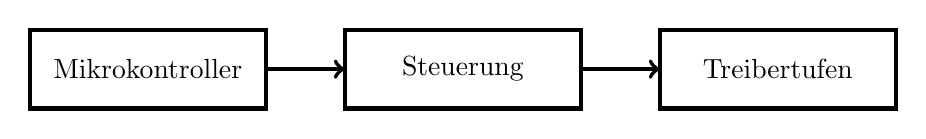
\begin{tikzpicture}
    		\draw[line width=1.5pt](0, 0) rectangle node{Mikrokontroller} (3, 1)  ;
    		\draw[line width=1.5pt, ->]	(3, 0.5) -- (4, 0.5);
    		\draw[line width=1.5pt](4, 0) rectangle node{Steuerung}(7, 1);
    		\draw[line width=1.5pt, ->]	(7, 0.5) -- (8, 0.5);
    		\draw[line width=1.5pt](8, 0) rectangle node{Treibertufen}(11, 1);
    		\end{tikzpicture}
    		\caption{Komponenten der Ansteuerung eines Schrittmotores}
    		\label{fig:ansteuerung}
    	\end{figure}
        Um die Ansteuerung zu realisieren, gibt es eine Vielzahl von integrierten Schaltkreisen. Diese unterscheiden sich wie folgt: 
        \begin{itemize}
        	\item \textbf{Interfaces:} Einzelanschlüsse, einfache Busschnittstellen oder Mikrokontrollerschnittstellen wie SPI, II2
        	\item \textbf{Steuerfunktionen:} Einzelne Schritte oder Bewegungsabläufe (Motion Control Functiona)
        	\item \textbf{Schaltungsintegration:} Steuerung und Treiberstufe als getrennte Schaltkreise, oder in einem Schaltkreis zusammengefasst. 
        \end{itemize}
        Der gewählte integrierte Schaltkreis ist der L6480 von STMicroelectronics. Dieser wird über die SPI Schnittstelle gesteuert und besitzt eine Motion Contol Engine. Die Treiberstufe wird extern realisiert. (Vgl. Kapitel \ref{sec:L6480} 
        
    \ifSTANDALONE
    \subsection{Treiberstufe}
    \fi
    \ifEMBED
    \subsubsection{Treiberstufe}
    \fi 
    	Wird ein Schrittmotor unipolar betrieben, so können die vier Wicklungen direkt mit Leistungsstufen angesteuert werden. Für den bipolaren Betrieb benötigt man für beide Wicklungen je eine H- Brücke. Die einfachste Methode ist es, den Strom nur durch den Wicklungswiderstand zu begrenzen. Der Nachteil ist, dass die Zeitkonstante durch den Wicklungswiderstand und der Induktivität bestimmt ist, und so bei höheren Schrittfrequenzen der gewünschte Strom und damit das Drehmoment nicht mehr erreicht wird. Deshalb wird ein zusätzlicher Vorwiderstand in Serie geschaltet, und so die Zeitkonstante verkleinert. Typische Verhältnisse sind vierfacher- oder fünffacher Widerstand, was eine vierfache bzw. fünffache Speisespannung voraussetzt. Diese Methode wiederum führt zu einer höheren Verlustleistung in den Widerständen. Im Ruhezustand ist es sinnvoll, den Strom soweit zu senken, dass das Haltemoment nicht unterschritten wird. Eine Spannungsumschaltung hat den weiteren Vorteil, dass so beim Anfahren eine steilere Stromkurve erreicht werden kann. (Vgl. \autoref{fig:spannungsumschaltung})
    	 \begin{figure}[h!]
    	 	\centering
    	 	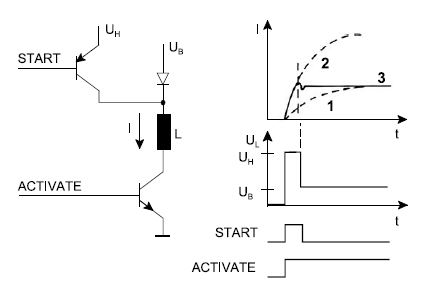
\includegraphics[width=8cm]{\EtPath/Bilder/spannungsumschaltung.jpg}
    	 	\caption{Spannungsumschaltung}
    	 	\label{fig:spannungsumschaltung}
    	 \end{figure}
    	Der Schrittmotor kann alternativ auch stromgesteuert betrieben werden. Dabei folgt der Stromverlauf dem Verlauf einer Referenzspannung (Sollwert). Der Stromverlauf wird auf den Sollwert geregelt. Die Betriebsspannung muss so nicht stabilisiert werden. \label{stromgesteuert} 
	
	
		
